% Cross-property unsupervised clustering section (consolidated view + PI rebalancing).
% Figures are tracked under figures/ (copied from the gitignored python/results/ tree).
% main.tex sets \graphicspath{{figures/}{./}}; this local \graphicspath is a fallback so
% the chapter also resolves figures when compiled on its own (e.g. via _smoke.tex).
\graphicspath{{figures/}{./}}
\subsection{Unsupervised clustering: a label-free cross-check}
\label{sec:eval-clustering}

The supervised attacks (Sections~\ref{sec:eval-pch}--\ref{sec:eval-spp}) assume an
adversary who can train on labeled executions. A weaker but assumption-free attacker
simply asks whether the on-chain gas features \emph{cluster} along the hidden property
with no supervision at all. Table~\ref{tab:clustering-summary} consolidates this attack
across all three properties: K-Means recovers essentially nothing, with ARI and NMI
within $\pm 0.02$ of zero for every DUO, PI, and SPP target. NMI values are interpreted
against the null finite-sample simulation in Section~\ref{sec:eval-nmi-sensitivity}.
The unsupervised attacker
agrees with the supervised verdict---privacy holds---as a second, label-free attack family
on the same dataset (Figure~\ref{fig:clust-summary}).

\begin{figure}[t]
  \centering
  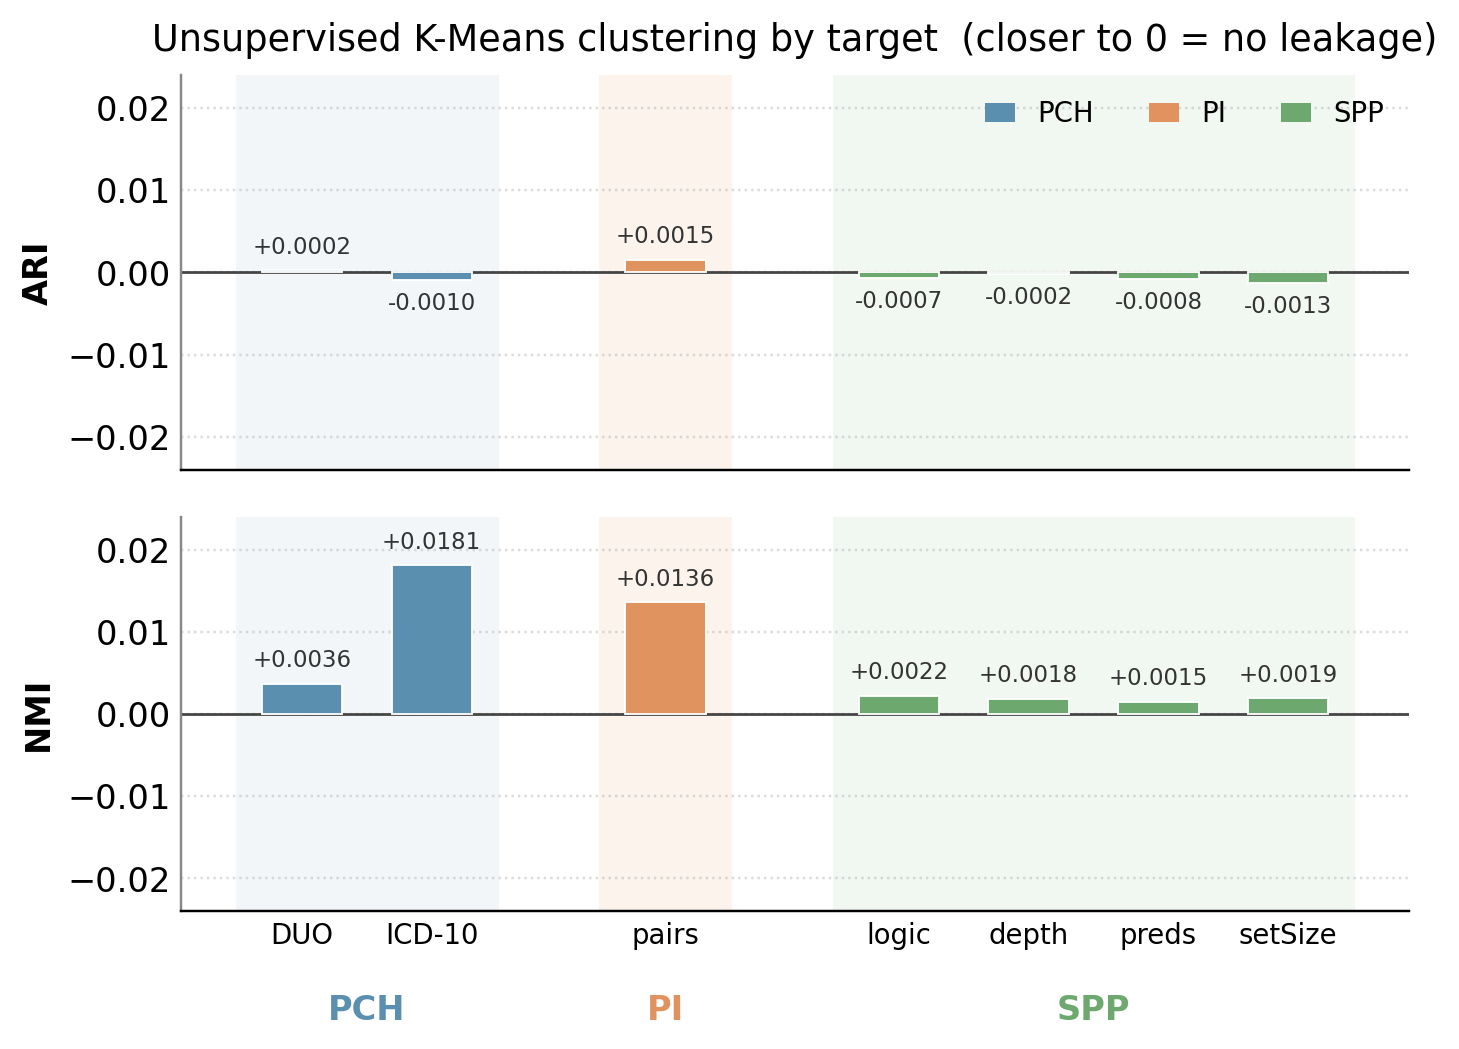
\includegraphics[width=\linewidth]{clustering_summary_unified.png}
  \caption{Unsupervised K-Means clustering across all three properties on a common
    axis: ARI (top) and NMI (bottom) for every PCH, PI, and SPP target. Every bar sits
    at the zero line---the natural gas clusters carry no information about the hidden
    label. SPP targets are abbreviated (logic: \texttt{logicStructure}; depth:
    \texttt{nestingDepth}; preds: \texttt{predicateCount}; setSize: \texttt{setSize}).
    NMI is read against the null finite-sample simulation in
    Section~\ref{sec:eval-nmi-sensitivity}.}
  \label{fig:clust-summary}
\end{figure}

\paragraph{Removing sample-size confounds.} The clustering inputs are constructed to
avoid degenerate measurements. The naive PI pairs were severely imbalanced (executions in
a $1{:}30$ ratio), under which K-Means trivially fails and a low ARI/NMI would be
meaningless. We rebuild the pairs into balanced $30$-vs-$30$ contrasts, and guard the
result with a permutation baseline---NMI under shuffled labels, where no true signal can
exist---reporting the debiased NMI (observed minus baseline) and its empirical $p$-value.
The conclusion is unchanged (Section~\ref{sec:eval-pi}): the indistinguishability is a
property of the protocol, not of a degenerate measurement. The ablation in
Section~\ref{sec:eval-ablation} supplies the positive control: clustering significance
appears on the un-padded gas transcript and disappears after normalization.
